%%%%%%%%%%%%%%%%%%%%%%%%%%%%%%%%%%%%%%%%%%%%%%%%%%%%%%%%%%%%%%%%%%%%%
%
% CSCI 1430 Written Question Template
%
% This is a LaTeX document. LaTeX is a markup language for producing documents. 
% You will fill out this document, compile it into a PDF document, then upload the PDF to Gradescope. 
%
% To compile into a PDF on department machines:
% > pdflatex thisfile.tex
%
% If you do not have LaTeX, your options are:
% - VSCode extension: https://marketplace.visualstudio.com/items?itemName=James-Yu.latex-workshop
% - Online Tool: https://www.overleaf.com/ - most LaTeX packages are pre-installed here (e.g., \usepackage{}).
% - Personal laptops (all common OS): http://www.latex-project.org/get/ 
%
% If you need help with LaTeX, please come to office hours.
% Or, there is plenty of help online:
% https://en.wikibooks.org/wiki/LaTeX
%
% Good luck!
% Srinath and the 1430 staff
%
%%%%%%%%%%%%%%%%%%%%%%%%%%%%%%%%%%%%%%%%%%%%%%%%%%%%%%%%%%%%%%%%%%%%%
%
% How to include two graphics on the same line:
%
% \includegraphics[width=0.49\linewidth]{yourgraphic1.png}
% \includegraphics[width=0.49\linewidth]{yourgraphic2.png}
%
% How to include equations:
%
% \begin{equation}
% y = mx+c
% \end{equation}
%
% How to include code:
%
% \begin{python}
% def f(x):
%   return x
% \end{python}
%
%
%%%%%%%%%%%%%%%%%%%%%%%%%%%%%%%%%%%%%%%%%%%%%%%%%%%%%%%%%%%%%%%%%%%%%%%%%%%%%%%%%%%%%%%%%%%%%%%%

\documentclass[11pt]{article}

\usepackage[english]{babel}
\usepackage[utf8]{inputenc}
\usepackage{amssymb}
\usepackage{xcolor}
\usepackage[colorlinks = true,
            linkcolor = blue,
            urlcolor  = blue]{hyperref}
\usepackage[a4paper,margin=1.5in]{geometry}
\usepackage{stackengine,graphicx}
\usepackage{fancyhdr}
\setlength{\headheight}{15pt}
\usepackage{microtype}
\usepackage{times}
\usepackage[shortlabels]{enumitem}
\setlist[enumerate]{topsep=0pt}
\usepackage{amsmath}
\usepackage{framed}
\usepackage{mdframed}
\usepackage{xcolor}
\usepackage[most]{tcolorbox}
\usepackage{booktabs}

% a great python code format: https://github.com/olivierverdier/python-latex-highlighting
\usepackage{pythonhighlight}

\usepackage{trimclip,lipsum}

\frenchspacing
\setlength{\parindent}{0cm} % Default is 15pt.
\setlength{\parskip}{0.3cm plus1mm minus1mm}

\pagestyle{fancy}
\fancyhf{}
\lhead{Homework 3 Questions}
\rhead{CSCI 1430}
\lfoot{\textcolor{red}{\textbf{Only}
\ifcase\thepage
\or \textbf{instructions}
\or \textbf{A1 (a)}
\or \textbf{A1 (b)}
\or \textbf{A1 (c) - (d)}
\or \textbf{A2 (a) (i)}
\or \textbf{A2 (a) (ii), (b)}
\or \textbf{A2 (c)}
\or \textbf{A2 (c)}
\or \textbf{A2 (c)}
\or \textbf{A3 (a)}
\or \textbf{A3 (b)}
\or \textbf{A4 (a)}
\or \textbf{A4 (b)}
\or \textbf{A4 (c)}
\or \textbf{A4 (d)}
\or \textbf{A5 (a)}
\or \textbf{A5 (b) - (c)}
\or \textbf{discussion attendance}
\or \textbf{feedback}
\else
\textbf{[ERROR: PAGE MISALIGNMENT]}
\fi
\textbf{should be on this page}
}}
\rfoot{\thepage/19}

\date{}

\title{\vspace{-1cm}Homework 3 Questions}


\begin{document}
\maketitle
\vspace{-2cm}
\thispagestyle{fancy}

\section*{ Document Instructions}
\begin{itemize}
  \item 5 questions \textbf{[10 + 8 + 4 + 13 + 3 = 40 points + 2 bonus points]}.
  \item Fill all your answers within the answer boxes, and \textbf{please do NOT remove the answer box outlines}.
  \item Questions are highlighted in the \textbf{orange boxes}, bonus questions are highlighted in \textbf{blue boxes}, answers should be recorded in the \textbf{green boxes}.
  \item Include code, images, and equations where appropriate.
  \item To identify all places where your responses are expected, search for `TODO'.
  \item The answer box sizes have been set by the staff beforehand and will truncate your text if it goes beyond the limit. Please make sure your responses fit in the appropriate spaces. \textbf{Extra pages are not permitted unless otherwise specified.}
  \item Make sure your submission has the right number of pages to validate page alignment sanity (check the footer).
  \item Please make this document anonymous.
\end{itemize}

\section*{ Gradescope Instructions}
\begin{itemize}
  \item When you are finished, compile this document to a PDF and submit it directly to Gradescope. 
  \item The pages will be automatically assigned to the right questions on Gradescope \textit{assuming you do not add any unnecessary pages}. \textbf{Inconsistently assigned pages will lead to a deduction of 2 points per misaligned page (capped at a maximum 6 point deduction).}
\end{itemize}
\pagebreak



%%%%%%%%%%%%%%%%%%%%%%%%%%%%%%%%%%%
\pagebreak
\paragraph{Q1:} \textbf{[10 points]}
Suppose we have a quadrilateral $ABCD$ and a transformed version $A'B'C'D'$ as seen in the image below.

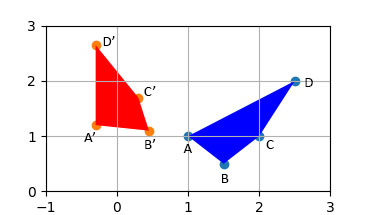
\includegraphics[width=\textwidth * 5/10]{images/quadrilaterals.jpg}

\begin{equation}
\begin{split}
A&=(1, 1)\\
B&=(1.5, 0.5)\\
C&=(2, 1)\\
D&=(2.5, 2)
\end{split}
\quad\quad\quad
\begin{split}
A'&=(-0.3, 1.3)\\
B'&=(0.5, 1.1)\\
C'&=(0.3, 1.8)\\
D'&=(-0.3, 2.6)
\end{split}
\end{equation}

Let's assume that each point in $ABCD$ was approximately mapped to its corresponding point in $A'B'C'D'$ by a $2\times2$ transformation matrix $\mathcal{M}$.

e.g. if $X = \begin{pmatrix} x \\ y \end{pmatrix}$ and $X' = \begin{pmatrix} x' \\ y' \end{pmatrix}$, and $\mathcal{M} = \begin{pmatrix} m_{1,1} & m_{1,2} \\ m_{2,1} & m_{2,2} \end{pmatrix}$

then $\begin{pmatrix} m_{1,1} & m_{1,2} \\ m_{2,1} & m_{2,2} \end{pmatrix} \times \begin{pmatrix} x \\ y \end{pmatrix} \approx \begin{pmatrix} x' \\ y'  \end{pmatrix}$

We would like to approximate $\mathcal{M}$ using least squares for linear regression.

\begin{enumerate}[(a)]
\item \textbf{[1 point]} 
\begin{tcolorbox}[colback=orange!5!white,colframe=orange!75!black]
Rewrite the equation $\mathcal{M} \times X \approx X'$ into a pair of linear equations by expanding the matrix multiplication.
\end{tcolorbox}

\begin{tcolorbox}[colback=white!5!white,colframe=green!75!black]
\setbox0=\hbox{\parbox[t]{\textwidth}{
    %%%%%%% ANSWER STARTS HERE %%%%%%%%%%%%%%%%%%%%%%%%%%%%
        
    TODO: Replace each of the `$\_\_$' below with $x, y, x', y',$ or $0$.
    \begin{align*}
    \begin{cases}
        \_\_m_{1,1} + \_\_m_{1,2} + \_\_m_{2,1} + \_\_m_{2,2} = \_\_
        \\\_\_m_{1,1} + \_\_m_{1,2} + \_\_m_{2,1} + \_\_m_{2,2} = \_\_
    \end{cases}
    \end{align*}
        
    %%%%%%% ANSWER ENDS HERE %%%%%%%%%%%%%%%%%%%%%%%%%%%%%%
    }}
\clipbox{0pt \dimexpr\dp0-4\baselineskip\relax{} 0in 0pt}{\copy0}
\end{tcolorbox}

\item \textbf{[2 points]}
With the quadrilaterals in question, there are 4 points that transform so we should expect to see 8 such equations (2 for each point) that use the transformation equation $\mathcal{M}$.

From these pairs of equations for each $x$-$x'$ correspondence, we can construct a matrix $\mathcal{Q}$ and column vector $b$ that satisfy
\begin{align*}
    \mathcal{Q} \times \begin{pmatrix} m_{1,1} \\ m_{1,2} \\ m_{2,1} \\ m_{2,2} \\ \end{pmatrix} = b
\end{align*}

\emph{Note:} Systems of linear equations are typically written in the form $\mathcal{A} \times x = b$, but since we have already defined $\mathcal{A}$ and $x$, we're writing it as $\mathcal{Q} \times m = b$

\begin{tcolorbox}[colback=orange!5!white,colframe=orange!75!black]
Find $\mathcal{Q}$ and $b$:\\

Replace each of the `$\_\_$' below with a $0$ or a coordinate value from $ABCD$ and $A'B'C'D'$.
\end{tcolorbox}

\begin{tcolorbox}[colback=white!5!white,colframe=green!75!black]
\setbox0=\hbox{\parbox[t]{\textwidth}{
    %%%%%%% ANSWER STARTS HERE %%%%%%%%%%%%%%%%%%%%%%%%%%%%
        
    TODO: your answer for (b) here
    \begin{align*}
        \begin{pmatrix} 
        \_\_ & \_\_ & \_\_ & \_\_ \\ 
        \_\_ & \_\_ & \_\_ & \_\_ \\ 
        \_\_ & \_\_ & \_\_ & \_\_ \\ 
        \_\_ & \_\_ & \_\_ & \_\_ \\ 
        \_\_ & \_\_ & \_\_ & \_\_ \\ 
        \_\_ & \_\_ & \_\_ & \_\_ \\ 
        \_\_ & \_\_ & \_\_ & \_\_ \\ 
        \_\_ & \_\_ & \_\_ & \_\_
        \end{pmatrix} 
        \times \begin{pmatrix} m_{1,1} \\ m_{1,2} \\ m_{2,1} \\ m_{2,2} \\ \end{pmatrix} 
        = \begin{pmatrix} 
        \_\_ \\ 
        \_\_ \\ 
        \_\_ \\ 
        \_\_ \\ 
        \_\_ \\ 
        \_\_ \\ 
        \_\_ \\ 
        \_\_ 
        \end{pmatrix}
    \end{align*}
        
    %%%%%%% ANSWER ENDS HERE %%%%%%%%%%%%%%%%%%%%%%%%%%%%%%
    }}
\clipbox{0pt \dimexpr\dp0-10\baselineskip\relax{} 0in 0pt}{\copy0}
\end{tcolorbox}

\item \textbf{[1 point]} Our problem is now over-constrained, so we want to find values for $m_{i,j}$ that minimize the squared error between the approximated values for $X'$ and the real $X'$ values, i.e., we want to minimize $||\mathcal{Q} \times m - b||$. 
\begin{align*}
\intertext{To do this we use singular value decomposition to find the pseudoinverse of $\mathcal{Q}$, written as $\mathcal{Q}^\dagger$. We then multiply it by both sides, giving us:}
 \mathcal{Q}^\dagger \mathcal{Q}m &= \mathcal{Q}^\dagger b\\
 \quad m &\approx \mathcal{Q}^\dagger b.
\end{align*}

Thankfully, the computer can do all of this for us! \texttt{numpy.linalg.lstsq()} takes in our $\mathcal{Q}$ matrix and $b$ vector, and returns approximations for $m$. Plug the values you wrote in part (c) into that function and write the returned $\mathcal{M}$ matrix here.

\textit{Note:} You may need to reshape your output from \texttt{linalg.lstsq} to get the right dimensions.

\begin{tcolorbox}[colback=orange!5!white,colframe=orange!75!black]
Replace each of the `$\_\_$' below with the value of $m_{i, j}$:
\end{tcolorbox}

\begin{tcolorbox}[colback=white!5!white,colframe=green!75!black]
\setbox0=\hbox{\parbox[t]{\textwidth}{
    %%%%%%% ANSWER STARTS HERE %%%%%%%%%%%%%%%%%%%%%%%%%%%%
        
    TODO: your answer for (c) here
    \begin{align*}
        M = \begin{pmatrix} m_{1,1} & m_{1,2} \\ m_{2,1} & m_{2,2} \end{pmatrix} = \begin{pmatrix} \_\_ & \_\_ \\ \_\_ & \_\_ \end{pmatrix}
    \end{align*}
        
    %%%%%%% ANSWER ENDS HERE %%%%%%%%%%%%%%%%%%%%%%%%%%%%%%
    }}
\clipbox{0pt \dimexpr\dp0-4\baselineskip\relax{} 0in 0pt}{\copy0}
\end{tcolorbox}

\item \textbf{[3 x 2 points]} Note that the least squares regression function that we use here is an approximation function, meaning that the values we derived for the transformation matrix are not exact. The same is true of our 8 point algorithm method of calculating the fundamental matrix.

\begin{tcolorbox}[colback=orange!5!white,colframe=orange!75!black]
Suppose there is some CV algorithm that uses an approximation such as the ones we learned about. Evaluate from the perspective of three stakeholders of your choice (e.g. the developer of the technology, the CEO of the company that develops the technology, a third party who uses your CV algorithm) how important transparency is surrounding margins of error. \textbf{[4-6 sentences]}
\end{tcolorbox}

\begin{tcolorbox}[colback=white!5!white,colframe=green!75!black]
\setbox0=\hbox{\parbox[t]{\textwidth}{
    %%%%%%% ANSWER STARTS HERE %%%%%%%%%%%%%%%%%%%%%%%%%%%%
        
    TODO: your answer for (d) here
        
    %%%%%%% ANSWER ENDS HERE %%%%%%%%%%%%%%%%%%%%%%%%%%%%%%
    }}
\clipbox{0pt \dimexpr\dp0-14\baselineskip\relax{} 0in 0pt}{\copy0}
\end{tcolorbox}

\end{enumerate}

%%%%%%%%%%%%%%%%%%%%%%%%%%%%%%%%%%%
% % Please leave the pagebreak
% \pagebreak
% \paragraph{A3 (continued):} Your answer here.

% If you really need extra space, uncomment here and use extra pages after the last question.
% Please refer here in your original answer. Thanks!
%\pagebreak
%\paragraph{AX.X Continued:} Your answer continued here.



%%%%%%%%%%%%%%%%%%%%%%%%%%%%%%%%%%%
% Please leave the pagebreak
\pagebreak
\paragraph{Q2:} \textbf{[8 points]}
In lecture, you've learned that cameras can be represented by intrinsic and extrinsic matrices. These matrices can be used to calculate the projections of points within a 3D world onto 2D image planes. For this, we use \emph{homogeneous coordinates}. The final $3\times4$ matrix is known as the \emph{camera matrix}.

Recall that the transformation can be represented by the following expression:
\begin{align*}
    \begin{pmatrix} 
    f_x & s & $0$ \\ 
    $0$ & f_y & $0$ \\ 
    $0$ & $0$ & $1$ \end{pmatrix} \times
    \begin{pmatrix} 
    r_{11} & r_{12} & r_{13} & t_x \\ 
    r_{21} & r_{22} & r_{23} & t_y \\  
    r_{31} & r_{32} & r_{33} & t_z
    \end{pmatrix} \times 
    \begin{pmatrix} 
    x \\ 
    y \\ 
    z \\ 
    $1$ \end{pmatrix}
    = w
    \begin{pmatrix}  u \\ v \\ $1$ \end{pmatrix}
\end{align*}
where $f$ is the focal point, $r$ is the rotation matrix, $t$ is the translation vector,  $w$ is some weighing/scaling factor, and $(u, v)$ is the position of the point in the real world $(x, y, z)$ projected on the 2D plane.

\begin{enumerate}[(a)]
\item \textbf{[2 points]}
For each of the following, you are given the camera specifications and a sample 3D point from the real world. 

\begin{tcolorbox}[colback=orange!5!white,colframe=orange!75!black]
Fill in the camera's intrinsic and extrinsic matrices; then, perform the multiplications and perspective division (unhomogenize) to find the 2D coordinate of the projected point on the image.
\end{tcolorbox}

\begin{enumerate} [(i)]
\item A camera with a focal length of 1 in both the $x$ and $y$ directions, a translation of 5 along the $x$-axis, and no skew or rotation.


\begin{tcolorbox}[colback=white!5!white,colframe=green!75!black]
\setbox0=\hbox{\parbox[t]{\textwidth}{
    %%%%%%% ANSWER STARTS HERE %%%%%%%%%%%%%%%%%%%%%%%%%%%%
        
    TODO: Fill in the \_\_ entries
    \begin{align*}
        & \qquad M_{\text{intrinsic}} \quad \times \qquad M_{\text{extrinsic}} \qquad  \times \; 
        \begin{pmatrix} 
            x  \\ 
            y  \\ 
            z  \\
            1
        \end{pmatrix} \\
        &= \begin{pmatrix} 
        \_\_ & \_\_ & $0$    \\  % <----- TODO: replace \_\_ %
        $0$ & \_\_ & $0$     \\  % <----- TODO: replace \_\_ %
        $0$ & $0$ & $1$ 
        \end{pmatrix} 
        \times
        \begin{pmatrix} 
        \_\_ & \_\_ & \_\_ & \_\_  \\ % <----- TODO: replace \_\_ %
        \_\_ & \_\_ & \_\_ & \_\_  \\ % <----- TODO: replace \_\_ %
        \_\_ & \_\_ & \_\_ & \_\_     % <----- TODO: replace \_\_ %
        \end{pmatrix} \times
        \begin{pmatrix} 
        $30$    \\ 
        $-20$   \\ 
        $10$    \\ 
        $1$ \end{pmatrix} \\
        &= \qquad \qquad \qquad \begin{pmatrix} 
        \_\_    \\   % <----- TODO: replace \_\_ %
        \_\_    \\   % <----- TODO: replace \_\_ %
        \_\_         % <----- TODO: replace \_\_ %
        \end{pmatrix} \\
        &= \qquad \quad \quad 
        \_\_         % <----- TODO: replace \_\_ %
        \times 
        \begin{pmatrix}  
        \_\_    \\   % <----- TODO: replace \_\_ %
        \_\_    \\   % <----- TODO: replace \_\_ %
        $1$ 
        \end{pmatrix}
    \end{align*}
        
    %%%%%%% ANSWER ENDS HERE %%%%%%%%%%%%%%%%%%%%%%%%%%%%%%
    }}
\clipbox{0pt \dimexpr\dp0-16\baselineskip\relax{} 0in 0pt}{\copy0}
\end{tcolorbox}


\item A camera with focal length of $2$ in both the $x$ and $y$ directions, a translation of $5$ along the $x$-axis, and no skew or rotation.
\begin{tcolorbox}[colback=white!5!white,colframe=green!75!black]
\setbox0=\hbox{\parbox[t]{\textwidth}{
    %%%%%%% ANSWER STARTS HERE %%%%%%%%%%%%%%%%%%%%%%%%%%%%
        
    TODO: Fill in the \_\_ entries
    \begin{align*}
        &= \begin{pmatrix} 
        \_\_ & \_\_ & $0$    \\  % <----- TODO: replace \_\_ %
        $0$ & \_\_ & $0$     \\  % <----- TODO: replace \_\_ %
        $0$ & $0$ & $1$ 
        \end{pmatrix} 
        \times
        \begin{pmatrix} 
        \_\_ & \_\_ & \_\_ & \_\_  \\ % <----- TODO: replace \_\_ %
        \_\_ & \_\_ & \_\_ & \_\_  \\ % <----- TODO: replace \_\_ %
        \_\_ & \_\_ & \_\_ & \_\_     % <----- TODO: replace \_\_ %
        \end{pmatrix} \times
        \begin{pmatrix} 
        $30$    \\ 
        $-20$   \\ 
        $10$    \\ 
        $1$ \end{pmatrix} \\
        &= \qquad \qquad \qquad \begin{pmatrix} 
        \_\_    \\   % <----- TODO: replace \_\_ %
        \_\_    \\   % <----- TODO: replace \_\_ %
        \_\_         % <----- TODO: replace \_\_ %
        \end{pmatrix} \\
        &= \qquad \quad \quad 
        \_\_         % <----- TODO: replace \_\_ %
        \times 
        \begin{pmatrix}  
        \_\_    \\   % <----- TODO: replace \_\_ %
        \_\_    \\   % <----- TODO: replace \_\_ %
        $1$ 
        \end{pmatrix}
    \end{align*}
        
    %%%%%%% ANSWER ENDS HERE %%%%%%%%%%%%%%%%%%%%%%%%%%%%%%
    }}
\clipbox{0pt \dimexpr\dp0-12\baselineskip\relax{} 0in 0pt}{\copy0}
\end{tcolorbox}

\end{enumerate}
\item \textbf{[2 points]}

\begin{tcolorbox}[colback=orange!5!white,colframe=orange!75!black]
Compare the two image coordinates you've calculated in parts a and b. Explain how each parameter affects the final image coordinate. \textbf{[2-3 sentences]}
\end{tcolorbox}

\begin{tcolorbox}[colback=white!5!white,colframe=green!75!black]
\setbox0=\hbox{\parbox[t]{\textwidth}{
    %%%%%%% ANSWER STARTS HERE %%%%%%%%%%%%%%%%%%%%%%%%%%%%
        
    TODO: Your answer to (b) here.
        
    %%%%%%% ANSWER ENDS HERE %%%%%%%%%%%%%%%%%%%%%%%%%%%%%%
    }}
\clipbox{0pt \dimexpr\dp0-12\baselineskip\relax{} 0in 0pt}{\copy0}
\end{tcolorbox}

%%%%%%%%%%%%%%%%%%%%%%%%%%%%%%%%%%%
% \paragraph{A4a:} Your answer here.
% Uncomment the stencil below and fill in your solution.

% \begin{enumerate}[(a)]

% \item

% \end{enumerate}

% \begin{enumerate}[(b)]

% \item

% \begin{python}
% # Your code here
% \end{python}

% \includegraphics[width=0.5\linewidth]{yourscreenshot.png}

% \end{enumerate}

%%%%%%%%%%%%%%%%%%%%%%%%%%%%%%%%%%%
% Please leave the pagebreak
\item \textbf{[1 + 3 points]}
In the questions folder, we've provided stencil code for a camera simulation in \texttt{camera\_simulation.py}. Given a camera matrix, the simulator visualizes an image that a camera would produce. 

\begin{tcolorbox}[colback=orange!5!white,colframe=orange!75!black]
Please implement \texttt{calculate\_camera\_matrix()} by calculating the camera matrix using the parameters given in the code (see stencil for more detail). When successful, you will see a bunny rendered as dots (see below). Paste your code for this function and attach a screenshot of the working demo once you finish. Play around with the sliders to see how different parameters affect the projection!
\end{tcolorbox}

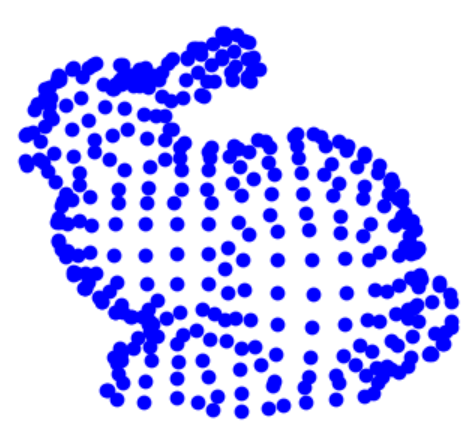
\includegraphics[width=0.5\linewidth]{images/bunny.png}

\begin{tcolorbox}[enhanced jigsaw,breakable,pad at break*=1mm,colback=white!5!white,colframe=green!75!black,height fixed for=all]
    %%%%%%% ANSWER STARTS HERE %%%%%%%%%%%%%%%%%%%%%%%%%%%%
    
    
\includegraphics[width=0.5\textwidth,height=7cm,keepaspectratio]{images/TODO_demo_screenshot.png}

        
    \begin{python}
import numpy as np
import matplotlib.pyplot as plt
from mpl_toolkits import mplot3d
from matplotlib.widgets import Slider, Button

# Initial random matrices
initial_intrinsic_matrix_to_replace = np.random.rand(3,3)
initial_extrinsic_matrix_to_replace = np.random.rand(3,4)
initial_camera_matrix_to_replace = np.random.rand(3,4)

# Setting up the point cloud
file_data_path= "./bunny.xyz"
point_cloud = np.loadtxt(file_data_path, skiprows=0, max_rows=1000000)
# center it
point_cloud -= np.mean(point_cloud,axis=0)
# homogenize
point_cloud = np.concatenate((point_cloud, np.ones((point_cloud.shape[0], 1))), axis=1)
# move it in front of the camera
point_cloud += np.array([0,0,-0.15,0])

def calculate_camera_matrix(tx, ty, tz, alpha, beta, gamma, fx, fy, skew, u, v):
    """
    This function should calculate the camera matrix using the given
    intrinsic and extrinsic camera parameters.
    We recommend starting with calculating the intrinsic matrix (refer to lecture 8).
    Then calculate the rotational 3x3 matrix by calculating each axis separately and
    multiply them together.
    Finally multiply the intrinsic and extrinsic matrices to obtain the camera matrix.
    :params tx, ty, tz: Camera translation from origin
    :param alpha, beta, gamma: rotation about the x, y, and z axes respectively
    :param fx, fy: focal length of camera
    :param skew: camera's skew
    :param u, v: image center coordinates
    :return: [3 x 4] NumPy array of the camera matrix, [3 x 4] NumPy array of the intrinsic matrix, [3 x 4] NumPy array of the extrinsic matrix
    """
    ########################
    # TODO: Your code here #
    # Hint: Calculate the rotation matrices for the x, y, and z axes separately.
    # Then multiply them to get the rotational part of the extrinsic matrix.
    ########################
    return (initial_camera_matrix_to_replace, 
    initial_intrinsic_matrix_to_replace, 
    initial_extrinsic_matrix_to_replace)

def find_coords(camera_matrix):
    """
    This function calculates the coordinates given the student's calculated camera matrix.
    Normalizes the coordinates.
    Already implemented.
    """
    coords = np.matmul(camera_matrix, point_cloud.T)
    return coords / coords[2]
    
    
    
    
    
    
    
    
    
    
    
    
    
    ################################################
    # YOU MAY USE THIS ADDITIONAL PAGE
    
    # WARNING: IF YOU DON'T END UP USING THIS PAGE
    # KEEP THESE COMMENTS TO MAINTAIN PAGE ALIGNMENT
    ################################################
    \end{python}
    %%%%%%% ANSWER ENDS HERE %%%%%%%%%%%%%%%%%%%%%%%%%%%%
\end{tcolorbox}

% \begin{tcolorbox}[colback=white!5!white,colframe=green!75!black]
%     \clipbox{0pt \dimexpr\dp0-1\baselineskip\relax{} 0in 0pt}{\copy0}
% \end{tcolorbox}


% \paragraph{A4b:} Your answer here.



%%%%%%%%%%%%%%%%%%%%%%%%%%%%%%%%%%%
\pagebreak
\paragraph{Q3:} \textbf{[4 points]} Given a stereo pair of cameras:
\begin{enumerate} [(a)]
\item \textbf{[2 points]} 
\begin{tcolorbox}[colback=orange!5!white,colframe=orange!75!black]
Briefly describe triangulation (using an image might be helpful) \textbf{[3-4 sentences]}
\end{tcolorbox}

\begin{tcolorbox}[colback=white!5!white,colframe=green!75!black]
\setbox0=\hbox{\parbox[t]{\textwidth}{
    %%%%%%% ANSWER STARTS HERE %%%%%%%%%%%%%%%%%%%%%%%%%%%%
    TODO: Your answer to (a) here.
    
    % OPTIONAL: Include your image here! This is not required.
    % \includegraphics[width=0.5\textwidth,height=7cm,keepaspectratio]{}
        
        
    %%%%%%% ANSWER ENDS HERE %%%%%%%%%%%%%%%%%%%%%%%%%%%%%%
    }}
\clipbox{0pt \dimexpr\dp0-20\baselineskip\relax{} 0in 0pt}{\copy0}
\end{tcolorbox}

\item \textbf{[2 points]} 
\begin{tcolorbox}[colback=orange!5!white,colframe=orange!75!black]
Why is it not possible to find an absolute depth for each point when we don't have calibration information for our cameras? Note that absolute depth refers to depth with respect to the camera as opposed to relative depth, which is with respect to another object in the scene. \textbf{[3 - 4 sentences]}
\end{tcolorbox}
\begin{tcolorbox}[colback=white!5!white,colframe=green!75!black]
\setbox0=\hbox{\parbox[t]{\textwidth}{
    %%%%%%% ANSWER STARTS HERE %%%%%%%%%%%%%%%%%%%%%%%%%%%%
        
    TODO: Your answer to (b) here.
        
    %%%%%%% ANSWER ENDS HERE %%%%%%%%%%%%%%%%%%%%%%%%%%%%%%
    }}
\clipbox{0pt \dimexpr\dp0-14\baselineskip\relax{} 0in 0pt}{\copy0}
\end{tcolorbox}

\end{enumerate}

\end{enumerate}

%%%%%%%%%%%%%%%%%%%%%%%%%%%%%%%%%%%
% \paragraph{A5:} Your answer here.
% Uncomment the stencil below and fill in your solution.

% \begin{enumerate}[(a)]

% \item

% \item

% \end{enumerate}


%%%%%%%%%%%%%%%%%%%%%%%%%%%%%%%%%%%
\pagebreak
\paragraph{Q4:} \textbf{[13 points]}
Given the algorithms that we've learned in computer vision, we know that whether we can find/calculate the essential matrix, the fundamental matrix, or both depends on the setup of the cameras and images. You are given three datasets of an object of unknown geometry:

\begin{enumerate}[(i)]
\item A video circling the object;
\item A stereo pair of calibrated cameras capturing two images of the object; and
\item Two images we take of the object at two different camera poses (position and orientation) using the same camera but with different lens zoom settings.
\end{enumerate}

\begin{enumerate}[(a)]
\item \textbf{[3 $\times$ 1 points]}
\begin{tcolorbox}[colback=orange!5!white,colframe=orange!75!black]
For each of the above setups, what calculations can we perform?
\end{tcolorbox}
\begin{enumerate}[(i)]
\item
Setup 1

\begin{tcolorbox}[colback=white!5!white,colframe=green!75!black]
\setbox0=\hbox{\parbox[t]{\textwidth}{
    %%%%%%% ANSWER STARTS HERE %%%%%%%%%%%%%%%%%%%%%%%%%%%%
        
    TODO: Select the right option:

    \begin{tabular}[h]{lc}
        \bottomrule
            Essential Matrix & $\square$ \\
            Fundamental Matrix & $\square$ \\
            Both & $\square$ \\
        \toprule
    \end{tabular}
        
    %%%%%%% ANSWER ENDS HERE %%%%%%%%%%%%%%%%%%%%%%%%%%%%%%
    }
    }
\clipbox{0pt \dimexpr\dp0-4\baselineskip\relax{} 0in 0pt}{\copy0}
\end{tcolorbox}

\item Setup 2
\begin{tcolorbox}[colback=white!5!white,colframe=green!75!black]
\setbox0=\hbox{\parbox[t]{\textwidth}{
    %%%%%%% ANSWER STARTS HERE %%%%%%%%%%%%%%%%%%%%%%%%%%%%
        
    TODO: Select the right option:

    \begin{tabular}[h]{lc}
        \bottomrule
            Essential Matrix & $\square$ \\
            Fundamental Matrix & $\square$ \\
            Both & $\square$ \\
        \toprule
    \end{tabular}
        
    %%%%%%% ANSWER ENDS HERE %%%%%%%%%%%%%%%%%%%%%%%%%%%%%%
    }}
\clipbox{0pt \dimexpr\dp0-4\baselineskip\relax{} 0in 0pt}{\copy0}
\end{tcolorbox}

\item Setup 3
\begin{tcolorbox}[colback=white!5!white,colframe=green!75!black]
\setbox0=\hbox{\parbox[t]{\textwidth}{
    %%%%%%% ANSWER STARTS HERE %%%%%%%%%%%%%%%%%%%%%%%%%%%%
        
    TODO: Select the right option:

    \begin{tabular}[h]{lc}
        \bottomrule
            Essential Matrix & $\square$ \\
            Fundamental Matrix & $\square$ \\
            Both & $\square$ \\
        \toprule
    \end{tabular}
        
    %%%%%%% ANSWER ENDS HERE %%%%%%%%%%%%%%%%%%%%%%%%%%%%%%
    }}
\clipbox{0pt \dimexpr\dp0-4\baselineskip\relax{} 0in 0pt}{\copy0}
\end{tcolorbox}
\end{enumerate}

\item \textbf{[3 $\times$ 1 points]} 
\begin{tcolorbox}[colback=orange!5!white,colframe=orange!75!black]
State an advantage and disadvantage of using each setup for depth reconstruction \textbf{[2 - 3 sentences]}
\end{tcolorbox}

\begin{enumerate}[(i)]
    \item Setup 1
    \begin{tcolorbox}[colback=white!5!white,colframe=green!75!black]
        \setbox0=\hbox{\parbox[t]{\textwidth}{
            %%%%%%% ANSWER STARTS HERE %%%%%%%%%%%%%%%%%%%%%%%%%%%%
                
            TODO: Your answer to (b) (i) here.
                
            %%%%%%% ANSWER ENDS HERE %%%%%%%%%%%%%%%%%%%%%%%%%%%%%%
            }}
        \clipbox{0pt \dimexpr\dp0-10\baselineskip\relax{} 0in 0pt}{\copy0}
    \end{tcolorbox}
    \item Setup 2
    \begin{tcolorbox}[colback=white!5!white,colframe=green!75!black]
        \setbox0=\hbox{\parbox[t]{\textwidth}{
            %%%%%%% ANSWER STARTS HERE %%%%%%%%%%%%%%%%%%%%%%%%%%%%
                
            TODO: Your answer to (b) (ii) here.
                
            %%%%%%% ANSWER ENDS HERE %%%%%%%%%%%%%%%%%%%%%%%%%%%%%%
            }}
        \clipbox{0pt \dimexpr\dp0-10\baselineskip\relax{} 0in 0pt}{\copy0}
    \end{tcolorbox}
    \item Setup 3
    \begin{tcolorbox}[colback=white!5!white,colframe=green!75!black]
        \setbox0=\hbox{\parbox[t]{\textwidth}{
            %%%%%%% ANSWER STARTS HERE %%%%%%%%%%%%%%%%%%%%%%%%%%%%
                
            TODO: Your answer to (b) (iii) here.
                
            %%%%%%% ANSWER ENDS HERE %%%%%%%%%%%%%%%%%%%%%%%%%%%%%%
            }}
        \clipbox{0pt \dimexpr\dp0-10\baselineskip\relax{} 0in 0pt}{\copy0}
    \end{tcolorbox}
\end{enumerate}

\item \textbf{[3 $\times$ 1 points]}
\begin{tcolorbox}[colback=orange!5!white,colframe=orange!75!black]
Name an application scenario for each of the different setups \textbf{[1 - 2 sentences]}
\end{tcolorbox}
\begin{enumerate}[(i)]
    \item Setup 1
    \begin{tcolorbox}[colback=white!5!white,colframe=green!75!black]
        \setbox0=\hbox{\parbox[t]{\textwidth}{
            %%%%%%% ANSWER STARTS HERE %%%%%%%%%%%%%%%%%%%%%%%%%%%%
                
            TODO: Your answer to (c) (i) here.
                
            %%%%%%% ANSWER ENDS HERE %%%%%%%%%%%%%%%%%%%%%%%%%%%%%%
            }}
        \clipbox{0pt \dimexpr\dp0-10\baselineskip\relax{} 0in 0pt}{\copy0}
    \end{tcolorbox}
    \item Setup 2
    \begin{tcolorbox}[colback=white!5!white,colframe=green!75!black]
        \setbox0=\hbox{\parbox[t]{\textwidth}{
            %%%%%%% ANSWER STARTS HERE %%%%%%%%%%%%%%%%%%%%%%%%%%%%
                
            TODO: Your answer to (c) (ii) here.
                
            %%%%%%% ANSWER ENDS HERE %%%%%%%%%%%%%%%%%%%%%%%%%%%%%%
            }}
        \clipbox{0pt \dimexpr\dp0-10\baselineskip\relax{} 0in 0pt}{\copy0}
    \end{tcolorbox}
    \item Setup 3
    \begin{tcolorbox}[colback=white!5!white,colframe=green!75!black]
        \setbox0=\hbox{\parbox[t]{\textwidth}{
            %%%%%%% ANSWER STARTS HERE %%%%%%%%%%%%%%%%%%%%%%%%%%%%
                
            TODO: Your answer to (c) (iii) here.
                
            %%%%%%% ANSWER ENDS HERE %%%%%%%%%%%%%%%%%%%%%%%%%%%%%%
            }}
        \clipbox{0pt \dimexpr\dp0-10\baselineskip\relax{} 0in 0pt}{\copy0}
    \end{tcolorbox}
\end{enumerate}
\item \textbf{[4 points]}
The differences between the collection methods for these three datasets are crucial in terms of what calculations are possible - and therein which applications they are most useful in.
\begin{tcolorbox}[colback=orange!5!white,colframe=orange!75!black] 
 From a non-technical standpoint, can you think of a scenario why you may prefer one of these data collection setups to another? Why is it important to know what data collection methods have been used to build a particular dataset? \textbf{[5-7 sentences]}
\end{tcolorbox}
\begin{tcolorbox}[colback=white!5!white,colframe=green!75!black]
\setbox0=\hbox{\parbox[t]{\textwidth}{
    %%%%%%% ANSWER STARTS HERE %%%%%%%%%%%%%%%%%%%%%%%%%%%%
        
    TODO: Your answer to (d) here.
    
    %%%%%%% ANSWER ENDS HERE %%%%%%%%%%%%%%%%%%%%%%%%%%%%%%
    }}
\clipbox{0pt \dimexpr\dp0-18\baselineskip\relax{} 0in 0pt}{\copy0}
\end{tcolorbox}
\end{enumerate}

%%%%%%%%%%%%%%%%%%%%%%%%%%%%%%%%%%%
% \paragraph{A6:} Your answer here.
% Uncomment the stencil below and fill in your solution.

% \begin{enumerate}[(a)]

% \item

% \item

% \item


%%%%%%%%%%%%%%%%%%%%%%%%%%%%%%%%%%%
% Please leave the pagebreak
% \pagebreak
% \paragraph{A6 (continued):} Your answer here.



%%%%%%%%%%%%%%%%%%%%%%%%%%%%%%%%%%%

% Please leave the pagebreak
\pagebreak
\paragraph{Q5:} \textbf{[3 points]} In two-view camera geometry, what do the following epipolar lines say about the cameras' relative positions? \textbf{[1 - 2 sentences each]}

\textit{Tip:} The Spring '22 course staff created an \href{https://browncsci1430.github.io/webpage/demos/stereo_camera_visualization/index.html}{interactive demo} to explore the different scenarios and get a better feel for epipolar geometry.

\begin{enumerate}[(a)]
\item \textbf{[1 point]} 
\begin{tcolorbox}[colback=orange!5!white,colframe=orange!75!black]
Radiate out of a point on the image plane.
\end{tcolorbox}

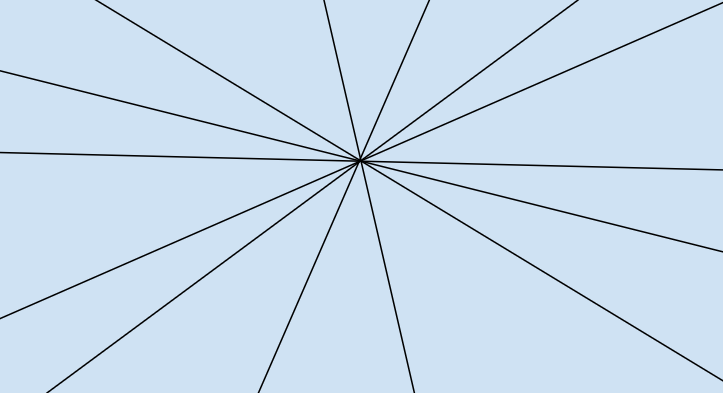
\includegraphics[width = 0.5\linewidth]{images/epipolarlines-a.PNG}
\begin{tcolorbox}[colback=white!5!white,colframe=green!75!black]
\setbox0=\hbox{\parbox[t]{\textwidth}{
    %%%%%%% ANSWER STARTS HERE %%%%%%%%%%%%%%%%%%%%%%%%%%%%
        
    TODO: Your answer to (a) here.
        
    %%%%%%% ANSWER ENDS HERE %%%%%%%%%%%%%%%%%%%%%%%%%%%%%%
    }}
\clipbox{0pt \dimexpr\dp0-8\baselineskip\relax{} 0in 0pt}{\copy0}
\end{tcolorbox}

\item \textbf{[1 point]}
\begin{tcolorbox}[colback=orange!5!white,colframe=orange!75!black]
Converge to a point outside of the image plane.
\end{tcolorbox}


\includegraphics[width = 0.5\linewidth]{images/epipolarlines-b.PNG}

\begin{tcolorbox}[colback=white!5!white,colframe=green!75!black]
\setbox0=\hbox{\parbox[t]{\textwidth}{
    %%%%%%% ANSWER STARTS HERE %%%%%%%%%%%%%%%%%%%%%%%%%%%%
        
    TODO: Your answer to (b) here.
        
    %%%%%%% ANSWER ENDS HERE %%%%%%%%%%%%%%%%%%%%%%%%%%%%%%
    }}
\clipbox{0pt \dimexpr\dp0-8\baselineskip\relax{} 0in 0pt}{\copy0}
\end{tcolorbox}

\item \textbf{[1 point]} 
\begin{tcolorbox}[colback=orange!5!white,colframe=orange!75!black]

% OLD QUESTION:
%What might you need to change about your fundamental matrix calculations if you obtained the following epipolar lines?%

Notice the misalignment of the epipolar lines in the image below? What went wrong in the calculation of the fundamental matrix and how can we fix it?

\textit{Hint:} Check slides from the lecture on stereo geometry.
\end{tcolorbox}

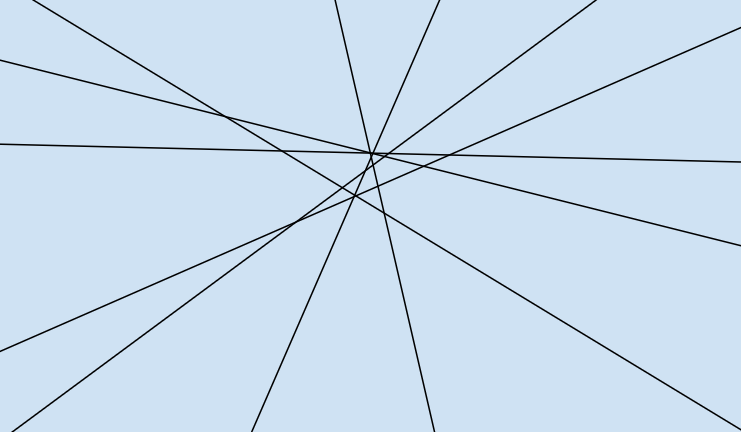
\includegraphics[width = 0.5\linewidth]{images/epipolarlines-c.PNG}
\begin{tcolorbox}[colback=white!5!white,colframe=green!75!black]
\setbox0=\hbox{\parbox[t]{\textwidth}{
    %%%%%%% ANSWER STARTS HERE %%%%%%%%%%%%%%%%%%%%%%%%%%%%
        
    TODO: Your answer to (c) here.
        
    %%%%%%% ANSWER ENDS HERE %%%%%%%%%%%%%%%%%%%%%%%%%%%%%%
    }}
\clipbox{0pt \dimexpr\dp0-8\baselineskip\relax{} 0in 0pt}{\copy0}
\end{tcolorbox}
\end{enumerate}



\pagebreak
\section*{Discussion Attendance:}
\paragraph{Extra Credit:} \textbf{[2 points]}

Please mark this box only if you've attended the discussion session in person.

\begin{tabular}[h]{ll}
$\square$ & I attended the discussion session on DATE \\
\end{tabular}

%%%%%%%%%%%%%%%%%%%%%%%%%%%%%%%%%%%
\pagebreak
\section*{Feedback? (Optional)}
Please help us make the course better. If you have any feedback for this assignment, we'd love to hear it!



\end{document}